\documentclass[aps,prb,twocolumn,letterpaper,twoside,nobalancelastpage,groupedaddress,amsmath,amssymb,floatfix,citeautoscript]{revtex4-1}
%\usepackage{geometry}       
%\geometry{letterpaper}     
%\usepackage[parfill]{parskip}    % Activate to begin paragraphs with an empty line rather than an indent
\usepackage{graphicx}
\usepackage{bm} %bold math symbols
\usepackage{times}
\usepackage{graphicx}
\usepackage{outlines}             
%\usepackage{amssymb}
\usepackage[caption=false]{subfig}
%\usepackage{mathtools}
\usepackage{color}
\definecolor{darkred}{rgb}{0.6,0.,0.}
\definecolor{darkgreen}{rgb}{0.,0.5,0.}
\definecolor{darkblue}{rgb}{0.,0.,0.6}

\usepackage{framed}

%\usepackage[square,numbers,sort,merge]{natbib}
\usepackage[
breaklinks,
colorlinks=true,
linkcolor=darkred,
citecolor=darkgreen,
urlcolor=darkblue]{hyperref}
%\usepackage{doi}

% \DeclareMathOperator{\tr}{tr}
% \DeclareMathOperator{\erf}{Erf}

\DeclareGraphicsRule{.tif}{png}{.png}{`convert #1 `dirname #1`/`basename #1 .tif`.png}

\begin{document}


\def \Ns {\mathbb{N}}
\def \Rs {\mathbb{R}}
\def \Zs {\mathbb{Z}}
\def \Qs {\mathbb{Q}}
\def \Cs {\mathbb{C}}
\def \id {\mathbb{I}}

\def \bfq {{\bf q}}
\def \bfp {{\bf p}}
\def \bfx {{\bf x}}
\def \bfy {{\bf y}}
\def \bfz {{\bf z}}
\def \bfr {{\bf r}}
\def \bfk {{\bf k}}
\def \bfn {{\bf n}}
\def \bfb {{\bf b}}

%\def \hata {{a}}
%\def \hatadag {{a}^{\dagger}}

\def \hatq {\widehat{q}}
\def \hatp {\widehat{p}}
\def \hata {\widehat{a}}
\def \hatadag {\widehat{a}^{\dagger}}
%\def \hatb {\widehat{b}^\phantom{\dagger}}
%\def \hatbdag {\widehat{b}^{\dagger}}
\def \wtN {\widetilde{N}}

\def \ve {\varepsilon}
\def \vth {\vartheta}



\title{}
\author{David Bauer}
\email{dbauer@physics.ucla.edu}
\affiliation{Department of Physics and Astronomy, University of California at Los Angeles, 475 Portola Plaza, Los Angeles, California 90095, USA}

\author{Fenner Harper}
\affiliation{Department of Physics and Astronomy, University of California at Los Angeles, 475 Portola Plaza, Los Angeles, California 90095, USA}

\author{Rahul Roy}
\affiliation{Department of Physics and Astronomy, University of California at Los Angeles, 475 Portola Plaza, Los Angeles, California 90095, USA}

\date{\today}
\begin{abstract}
Abstract goes here.
% Recent work on the quantum Hall effect (QHE) in lattice models and other systems with non-trivial geometry has opened the question of the extent to the stability of quantum Hall states is dependent on Landau levels. We construct a lattice model that has as its continuum limit a Hamiltonian with purely quartic momentum dependence, yielding single-particle states different from Landau levels in which one may study the QHE. We study the spectrum and band structure of the lattice Hamiltonian and its continuum limit, as well as the fractional quantum Hall effect (FQHE) of interacting particles in these bands. 
\end{abstract}

% \pacs{0}

\maketitle
% \begin{outline}
% \1 Introduction
% \1 Effective continuum hamiltonians
% \1 The quartic model -- spectrum, band geometry, etc.
% \1 FQH physics in the quartic LLL
% \1 Discussion
% \end{outline}
\section{Introduction}
\subsection{Background and motivation}
The quantum Hall (QH) effects have provided a rich laboratory for a wide variety of condensed matter physics concepts for decades. In particular, they serve as important prototypes for the study of topologically ordered phases. Despite a huge body of literature on the QH effects and many successful theoretical developments, a ``unified theory'' of QH physics has not yet emerged. Some recent attempts to expand our range of understanding have focused on removing the standard simplification of introducing non-generic symmetries to the problem, for example rotational symmetry. Put slightly differently, this amounts to studying the QH effect in settings where the single-particle bands are not Landau levels (LL), as Landau levels have symmetries unnecessary for the stability of QH phases.

An extreme example of a system without the symmetries present in the standard two-dimensional electron gas (2DEG) setup is one in which electrons live on a lattice. Even in the regime in which may treat such a system with an effective continuum theory, effects like band mass anisotropy can spoil the non-generic symmetries. While lattice theories may lack the symmetries of the 2DEG, the effective continuum theory for a generic lattice theory will, at lowest order, be one of Landau levels. Thus, if we wish to study a less-symmetric continuum model, it seems we should not start with a lattice model.

In this work, we show how one may construct a family of toy models on a lattice that do not have Landau levels as their lowest-order continuum eigenstates. In other words, we obtain single-particle bands that cannot be treated as perturbations of Landau levels. 


This direction  has a natural connection to the single-mode approximation (SMA) employed in studying the bulk neutral excitations of fractional quantum Hall (FQH) fluids. The lowest energy branch of these excitations is the magnetoroton or Girvin-MacDonald-Platzman (GMP) mode. This is the relevant part of the spectrum if we are interested in the stability of the gap in FQH systems. The quadropolar nature of the GMP mode suggests that this mode should be sensitive to the geometry of a FQH liquid, particularly the presence or absence of rotational symmetry.

\subsection{Universality of Landau levels}
Consider a tight-binding lattice model for an electron in two dimensions in the presence of a uniform, perpendicular magnetic field; we will refer to such a system as a Harper-Hofstadter (HH) model.
We will assume that the lattice is inversion-symmetric, and that time reversal symmetry is unbroken when $B=0$.

\subsection{Relation to previous work}



% The quantum Hall (qH) effects have served as powerful motivating examples of the role of topology in condensed matter physics. In particular, the topological nature of qH phases explains their surprisingly robust universal properties, such as quantized transport coefficients. Several recent developments in qH physics have focused on the role of geometry in 


% In this article, we exhibit a family of tightbinding lattice models whose effective continuum hamiltonians have such generalized Landau level eigenstates. These hamiltonians are distinct from the Landau level hamiltonian in that they cannot be treated as perturbations around it. We study a particular case of 


% Since single-particle tightbinding models are amenable to exact diagonalization, we can numerically study topological and geometric properties of these bands as well as the physics of interacting particles projected onto the bands. We find that there is a gapped many-body phase consistent Laughlin-like phases of FCIs.
\clearpage
[The rest of this needs to be revised and completed.]
\section{Effective continuum hamiltonians}
We consider a single spinless particle moving in the periodic potential of an inversion-symmetric lattice. 
\begin{align*}
H = \sum_{\bfk}E(\bfk)\, c^{\dag}_{\bfk}c_{\bfk}.
\end{align*}
Since our lattice is inversion symmetric and we have not yet broken time reversal symmetry, $E(\mathbf{k}) = E(-\mathbf{k})$. We make the further assumption that $E$ has a global minimum at $k=0$. Taylor expanding $E(\mathbf{k})$ about this minimum, we have
\begin{align}
\label{equation:generic-dispersion}
E(\bfk) = \frac{1}{2}g_0^{ij}k_i k_j
+ \sum_{j=2}^{\infty}\sum_{m=0}^{2j} \Lambda_{j,m}~ k_x^m k_y^{2j-m}.
\end{align}

While this expansion will produce an arbitrary symmetric $g_0$, we may bring $g_0$ to diagonal form by a $GL(2,\mathbb{R})$ transformation.

% by a $GL(2,\mathbb{R})$ transformation $H_0$ can be reduced to three possible forms
We introduce a perpendicular magnetic field $B = \partial_x A_y - \partial_y A_x$. Working with a lattice in the tight-binding approximation with hopping amplitudes $t_{ij}$, this field is incoporated by the Peierls substitution
\begin{align*}
t_{ij} \rightarrow t_{ij}\exp\left[\frac{2\pi i}{\phi_0}\int_{i}^{j}\mathbf{A}\cdot\text{d}\boldsymbol{\ell}\right].
\end{align*}
After expanding, the effect on the dispersion (\ref{equation:generic-dispersion}) is the minimal substitution $\bfk \rightarrow \bfk - \frac{e\mathbf{A}}{c}$. In the Landau gauge with $\mathbf{A} = (0,B x)$, 
\begin{align*}
H = \frac{p^2 + \xi^2}{2m\ell^2} + \sum_{j=2}^{\infty}\sum_{m=0}^{2j} \frac{\Lambda_{j,m}}{\ell^{2j}}~ p^m \xi^{2j-m}.
\end{align*}
% \begin{align*}
% H = \frac{p^2}{2m} + \frac{\xi^2}{2m\ell^4} + \sum_{j=2}^{\infty}\sum_{m=0}^{2j} \Lambda_{j,m}~ p^m \left(\frac{\xi}{\ell^2}\right)^{2j-m}.
% \end{align*}
where $\ell = \hbar c / e B$ is the magnetic length and $\xi = \hbar(x - \ell^2 k_y)/\ell$


In the $\ell \rightarrow \infty$ limit corresponding to small magnetic field, the quadratic term, which we label $H_0$, dominates. Its eigenstates are the familiar Landau levels $\left|n,k_y\right>$ with eigenvalues $\epsilon_n = (\hbar/m \ell^2)\left(n + \frac{1}{2}\right)$. Since we have only assumed inversion symmetry of the dispersion, we expect that generic lattice bands will approach Landau levels in the $\ell\rightarrow \infty$  limit so long as the quadratic part of the Hamiltonian does not vanish identically.

If one or both quadratic terms do vanish, the continuum limit Hamiltonian will produce non-Landau level behavior to lowest order. While an exactly vanishing $H_0$ is an idealization, it is in principle possible to tune the parameters of the problem so that $H_0$ is negligible. To demonstrate this, we consider the Hamiltonian
\begin{align}
\label{perturbation-hamiltonian}
H = \frac{1}{\ell^4}H_1 + \frac{\lambda}{\ell^2} H_0 
\end{align}
Where $H_1$ is a homogeneous, quartic polynomial in components of $\bfp$, and $\lambda$ is a parameter. Each term in the Hamiltonian has been scaled to show $\ell$ dependence explicitly. We write the eigenstates of $H_1$ in a basis of Landau levels, 
\begin{align}
\label{landau-level-expansion}
\left|\tilde{n}\right> = \sum_{n=0}^{\infty} c_n \left|n\right>.
\end{align}
To establish quantitative bounds on observable effects of $H_0$, we treat the Landau level Hamiltonian $\lambda\ell^2 H_0$ as a perturbation and study the remainder terms of the zeroth order Taylor polynomials for the eigenstates and eigenvalues. With an error tolerance $\tau$, corrections to the $n$th energy eigenvalue from $H_0$ are unobservable if the parameter $\lambda$ obeys
\begin{align}
\label{equation-lambda-bound}
\lambda < \frac{\tau \epsilon_n}{\left<\tilde{n}\right|\!H_0\!\left|\tilde{n}\right>\ell^2}.
\end{align}
where $\epsilon_n$ is the $n$th eigenvalue of $H_1$. Since first order corrections to the eigenstates of $H$ vanish, (\ref{equation-lambda-bound}) provides the most conservative bound on $\lambda$; observable effects arising from corrections to states will also be negligible if (\ref{equation-lambda-bound}) is obeyed.

Generically, the quartic term $E_1$ can take three possible forms, 
\begin{align}
\label{dispersion-metric}
E^{(1)}_1 &= (g_1^{ab}k_a k_b) (g_2^{cd} k_c k_d)\\
E^{(2)}_1 &= (\mathbf{a}_1 \cdot \mathbf{k})(\mathbf{a}_2 \cdot \mathbf{k})(g_1^{ab}k_a k_b)\\
E^{(3)}_1 &= (\mathbf{a}_1 \cdot \mathbf{k})(\mathbf{a}_2 \cdot \mathbf{k})(\mathbf{a}_3 \cdot \mathbf{k})(\mathbf{a}_4 \cdot \mathbf{k})
\end{align}
where the $g_i$ are symmetric 2x2 matrices with $\text{det}~g_i > 0$, and the $a_i$ are elements of $\mathbb{R}^2$. In the case that we may neglect the quadratic term, only the first of these has a unique global minimum at $\bfk=0$, forcing the continuum limit dispersion to take this form. 

% If the quadratic term vanishes identically, then the lowest order term in the dispersion will be quartic. Keeping only this quartic term, the dispersion takes one of three possible forms
% \begin{align*}
% l
% \end{align*}
% The requirement that $E$ have a global minimum at $\bfk = 0$ restricts $E$ to take the first form only.

%%%%%%%%%%%%%%%%%%%%%%%%%%%%%%%%%%%%%%%%%%%%%%%%%%%%%
[ignore this \{]
\textbf{Finite difference approximations}
\begin{align*}
\Delta^2 f &= \frac{f(x-a) - 2f(x) + f(x+a)}{a^2}\\
\Delta^2 f - \partial^2 f &= \frac{a^2}{12}\partial^4f + O(a^4)
\end{align*}

\begin{align*}
\Delta^4 f &= \frac{f(x-2a) - 4f(x-a) + 6f(x) - 4f(x+a) + f(x+2a)}{a^4}\\
\Delta^4 f - \partial^4 f &= \frac{a^2}{6}\partial^6 f + O(a^4)
\end{align*}
[\}]

As a concrete demonstration of the preceding ideas, we study lattice realizations of two models with non-Landau level behavior.
We begin by considering the familiar Hofstadter model on a square lattice with nearest neighbor hopping amplitude $t_1$ and modify the model by including a next-nearest neighbor hopping with amplitude $t_2$ along the $x$ and $y$ directions. Setting the lattice spacing $a=1$ and writing the eigenstates $\psi(x = n,y) = e^{i k_y y}\psi_n$, the Harper eigenvalue equation for this model is
\begin{align}
\label{equation-quartic-harper}
&\varepsilon \psi_{n} = -t_1\left(\psi_{n+1} + \psi_{n-1}\right)\nonumber - t_2\left(\psi_{n+2} + \psi_{n-2}\right)\\
 -&2t_1\cos\left(\frac{1}{\ell^2}n - k_{y}\right)\psi_n\nonumber 
  -2t_2\cos\left(2 \frac{1}{\ell^2}n - 2k_{y}\right)\psi_n.
\end{align}
For $\ell$ large, we approximate $\psi_n$ by a continuum wavefunction $\psi(x)$, Taylor expanding both the finite differences and cosine terms. This yields the differential equation
\begin{align*}
 -&(1 + 4t)\frac{1}{\ell^2}\frac{d^2 \psi}{d \xi^2} + (1 + 4t)\frac{1}{\ell^2}\xi^2~\psi(\xi)\\ - &t\frac{1}{\ell^4}\frac{d^4 \psi}{d \xi^4} -\frac{\left(1 + 16t\right)}{12}\frac{1}{\ell^4}\xi^4~\psi(\xi) =  \tilde{\varepsilon}\psi(\xi)
\end{align*}
where $t=t_2/t_1$, $\xi=x/\ell$, and $\tilde{\varepsilon} = \varepsilon/t_1 + 4(1+t)$. With hopping amplitudes tuned so that $t = -\frac{1}{4}$, this becomes
\begin{align*}
&\frac{1}{4\ell^4}\frac{d^4 \psi}{d \xi^4}  + \frac{1}{4\ell^4}\xi^4~\psi(\xi) =  \tilde{\varepsilon}\psi(\xi).
\end{align*}
This is the Schrodinger eigenvalue equation for the Landau gauge Hamiltonian 
\begin{align*}
H_1 = \frac{1}{4\ell^4}\left(p^4 + \xi^4\right)
\end{align*}
corresponding to the dispersion $E_1(\bfk) = (k_x^4 + k_y^4)/4$. In the notation of $(\ref{dispersion-metric})$, one choice of $g_1$, $g_2$ is
\begin{align*}
g_1 = \frac{1}{2}\begin{pmatrix}1 &1/\sqrt{2}\\1/\sqrt{2} &1\end{pmatrix}, g_2 = \frac{1}{2}\begin{pmatrix}1 &-1/\sqrt{2}\\-1/\sqrt{2} &1\end{pmatrix}.
\end{align*}

A semi-classical argument applying the Bohr-Sommerfield quantization condition lets us estimate the behavior of the energy eigenvalues in the high energy limit. We write the classical energy of this system
\[
E = \frac{p^4+\xi^4}{4\ell^4}
\]
and impose the Bohr-Sommerfeld condition
\[
\int \text{d}\xi~p(\xi) \sim n \in \mathbb{Z}.
\]
This yields
\begin{align*}
E \sim \ell^{-4} n^2,
\end{align*}

To study the eigenvalues and eigenstates of this Hamiltonian further, we work in a basis of Landau levels $\{\left|n\right>\}$ and write the scaled position and momentum operators in terms of Landau level raising and lowering operators,
\begin{align*}
\xi = \frac{1}{\sqrt{2}}\left(a + a^{\dag}\right)\\
p = \frac{-i}{\sqrt{2}}\left(a - a^{\dag}\right)
\end{align*}
with $\left[a,a^{\dag}\right] = 1$ and $a\!\left|0\right> =0$.

[Spectrum of quartic Hamiltonian, etc....]

We now consider moving away from the fine-tuned case, letting $t = -1/4 + \delta$. The eigenvalue equation
\begin{align*}
-&\frac{4\delta}{\ell^2}\left[\frac{d^2 \psi}{d \xi^2} + \xi^2~\psi(\xi)\right]\\ + &\left(\frac{1}{4} - \delta\right)\frac{1}{\ell^4}\frac{d^4 \psi}{\partial \xi^4} -\left(\frac{1}{4} - \frac{4}{3}\delta\right)\frac{1}{\ell^4}\xi^4~\psi(\xi) =  \tilde{\varepsilon}\psi(\xi)
\end{align*}
now contains quadratic terms, and the corresponding Hamiltonian is of the form (\ref{perturbation-hamiltonian}) with $\lambda = 4\delta$. 

Using the bound (\ref{equation-lambda-bound}), we can establish a range for $\delta$ such that the bands of the lattice model are distinct from Landau levels in the continuum limit; for concreteness we restrict our attention to the lowest band $\left|\tilde{0}\right>$. Calculating $\epsilon_0$ and $\left<H_0\right>$ numerically using the finite subspace approximation described above, we find the condition
\begin{align*}
\delta \lesssim 0.086 \frac{\tau}{(\ell/a)^2},
\end{align*}
restoring the necessary factor of the lattice spacing $a$. We can relate this to experiment by calculating some typical experimental values of $\ell$.  
In a recent optical lattice simulation of the Hofstadter model, researchers achieved an effective $B\approx0.0441$ T magnetic field; the corresponding magnetic length, measured in units of the lattice spacing, is $\ell\approx0.0143 ~a$, so that 
\begin{align*}
\delta \lesssim 423~ \tau
\end{align*}
This represents the region of large lattice effects. As an example system closer to the continuum limit, we consider a GaAs heterostructure in a 30 T magnetic field. Here we have $\ell \approx 6.3\times10^{-4}~ a$, and
\begin{align*}
\delta \lesssim 1.36\times10^{-6}~ \tau
\end{align*}

% We begin by considering the familiar Hofstadter model on a square lattice with nearest neighbor hopping amplitude $t_1$ and modify the model by including a next-nearest neighbor hopping with amplitude $t_2$ along the $y$ direction only. This gives the modified Harper eigenvalue equation
% \begin{align}
% \label{equation-harper-2}
% &-\left(\psi_{n+1} + \psi_{n-1}\right)\nonumber -2\cos\left(\frac{a^2}{\ell^2}n - k_{y}\right)\psi_n\nonumber \\*
%   &-2\frac{t_2}{t_1}\cos\left(2 \frac{a^2}{\ell^2}n - 2k_{y}\right)\psi_n = \frac{\varepsilon}{t_1} \psi_{n}.
% \end{align}
% $2 \pi (\phi/\phi_0) = a^2/\ell^2$

% For $\ell/a$ large, we approximate this difference equation by a differential equation for $\psi(x)$,
% \begin{align*}
% &-\frac{\partial^2 \psi}{\partial x^2} - 2\cos\left(\frac{ax}{\ell^2}\right)\psi(x)\\ &-2\frac{t_2}{t_1}\cos\left(2 \frac{ax}{\ell^2}\right) \psi(x) = \left(\frac{\varepsilon}{t_1} + 2\right) \psi(x)
% \end{align*}

% We can further modify the Hofstadter model by including next-nearest neighbor hopping in both $x$ and $y$ directions. 



%%%%%%%%%%%%%%%%%%%%%%%%%%%%%%%
% Value of magnetic field, hopping parameters from experiments.







% \subsection{Background and motivation}
% \label{intro:background}
% %[FQHE and landau levels]

% Standard theories of the integer and fractional quantum Hall effects (IQHE and FQHE, respectively) are based on the single-particle Landau level orbits that arise in a 2-dimensional system in the presence of continuous Galilean and rotational symmetries. A prototypical example of such a theory is Laughlin's wavefunction for the $\nu = 1/m$ fractional quantum Hall states \cite{Laughlin:1983hk}, which employs the holomorphic structure of lowest Landau level (LLL) wavefunctions ultimately arising from these symmetries. Much recent literature has focused on the potential formation and properties of quantum Hall (QH) phases in the absence of such continuous symmetries. These developments lead to an understanding of the more universal aspects of QH systems, but also have the potential to elucidate features of QH states in lattice systems. 

% %[FCIS]

%  Time-reversal breaking lattice models with flattened bands may exhibit the FQHE when fractionally filled with interacting particles. Such models are known as fractional Chern insulators, and their study has led to recent interest in lattice FQH systems; recent work on these systems is reviewed in Refs \cite{Parameswaran:2013uf,Bergholtz:2013ue}. While these bands exhibit some properties of Landau levels essential to the appearance of the QHE, such as Chern number and flat energy dispersion, they are in general quite different from the Landau levels on which theories of the QHE are based. As yet, there is no general theory of FCI states at the level of generality of, for example, the Laughlin wavefunction. Other studies of the QHE in lattice systems and its relation to the topology of such systems include \textcite{Thouless:1982kq} and \textcite{Haldane:1988gh}. The QHE in the Hofstadter model specifically, especially in connection with atoms in optical lattice, is well-studied \cite{Sorensen:2005bt,Palmer:2006km,Hafezi:2007gz,Moller:2009ir,Kapit:2010ky,Sterdyniak:2012jo,Scaffidi:2014tg,Harper:2014vi}.

% % Due to the topological nature of the FQH states, one expects 
 
% %[Geometry and Hall viscosity]

% In addition to explicitly studying the appearance of the QHE in lattice bands, one can consider the effects of the lattice that persist in the continuum limit, for example band mass anisotropy; this naturally leads to a geometrical description of the single particle orbits based on a non-Euclidean metric tensor \cite{Yang:2012ab,Haldane:2016aa}. The quantum Hall effect in the presence of non-trivial geometry -- that is, a non-Euclidean metric -- is connected with the theory of Hall viscosity, which is the linear response of a system to variations in the metric tensor\cite{Avron:1995aa,Cho:2014aa}. As an example of a system in which one cannot apply the usual, Euclidean geometry of Landau levels, \textcite{Haldane:2016aa} studied the continuum single-particle Hamiltonian containing quartic momentum terms and its connection to the IQHE and Hall viscosity.

% %[Summary of our work]

% In this work, we exhibit a square lattice model that in the continuum limit yields a Hamiltonian that to lowest order is quartic in momentum. We expect that generically a lattice tight-binding Hamiltonian will have a quadratic Hamiltonian as its continuum limit, possibly with rotationally asymmetric cross-terms. In this case, terms higher order in momentum that arise in taking the continuum limit can be studied perturbatively. Since quadratic momentum terms vanish exactly in our model, the quartic terms and their rotational symmetry breaking effects cannot be treated as perturbations. We explicitly show how such a Hamiltonian may arise as the continuum limit of a lattice model, exhibit the connections between the lattice and continuum models, and study the formation of the FQHE by interacting particles in the lattice bands. The Hamiltonian we study is a modification of the well-known Hofstadter Hamiltonian, and we now provide a brief introduction the Hofstadter model and discuss its continuum limit. We will then discuss some generalities of the continuum quartic Hamiltonian before moving to our lattice model.

% \subsection{The Hofstadter model in small flux}
% \label{sec:intro-hof}
% We consider a two-dimensional tight binding model on a square lattice with perpendicular magnetic field $B=\partial_x A_y - \partial_y A_x$. Including just a nearest neighbor hopping term, the Hamiltonian for this system is the well-known Hofstadter Hamiltonian \cite{Harper:1955ft,Hofstadter:1976js}
% \[
% \label{eq-hof}
% H = -t_1 \sum_{\langle i j \rangle} \left[ c_{\bm{r}_i}^{\dagger} c_{\bm{r}_j} \exp\left(i\theta_{\bm{r}_i,\bm{r}_j}\right)  + \text{h.c.} \right]
% \]
% where $i$,$j$ run over the sites of a square lattice and
% \begin{equation*}
% \theta_{\bm{r}_i,\bm{r}_j}= \frac{2\pi}{\phi_0}\int_{\bfr_{i}}^{\bfr_{j}} \! \bf{A} \cdot \text{d} \bm{\ell}.
% \end{equation*}
% In the Landau gauge, this Hamiltonian leads to the Harper eigenvalue equation
% \[
% \label{eq-harper}
% -\psi_{n+1} - \psi_{n-1} -  2\cos(2 \pi n \phi/\phi_0 - k_{y}) \psi_{n} = \varepsilon \psi_{n}.
% \]
% Here we have set $t_1=1$. Following \cite{Harper:2014vi}, in the limit of small flux per plaquette, one can approximate this difference equation by a continuum differential equation
% \begin{align*}
% -\frac{1}{2}\frac{d^2\psi}{dx^2} - \cos\left(2\pi x \phi/\phi_0 \right)\psi(x) = \frac{\varepsilon}{2}\psi(x)
% \end{align*}
% and expand the cosine term to second order in $\phi$. Setting $\omega \equiv 2\pi\phi/\phi_0$, $\tilde{\varepsilon} \equiv \frac{\varepsilon +2}{2}$, this gives
% \begin{align}
% \label{eq:landau-hamiltonian}
% -\frac{1}{2}\frac{d^2\psi}{dx^2} + \frac{1}{2}\omega^2 x^2~\psi(x) = \tilde{\varepsilon}\psi(x) ,
% \end{align}
% which we recognize as the Schr{\"o}dinger euqation for a harmonic oscillator as appears in the Landau level problem. We note that for small flux, the energy depends linearly on $\omega$ and thus $\phi$, as seen in the small-flux behavior of the Hofstadter ``butterfly'' spectral plot.

% % \subsection{Summary}
% % In the next section of this work, we will introduce the model of interest and study some of its properties, both in the lattice case and in the continuum limit. We introduce an interaction potential and diagonalize its projection to the lattice bands to study the formation of the fractional quantum Hall effect in these bands.

% \subsection{Chern band geometry}

% \subsection{Continuum quartic Hamiltonian}
% \label{sec:intro-quartic}
% We now discuss the continuum Hamiltonian with diagonal quartic momentum terms for an electron moving in 2D in the presence of a perpendicular magnetic field,
% \begin{align}
% \label{eq:quartic-continuum-hamiltonian}
% H = \frac{1}{4m^3}\bm{\pi}^4,
% \end{align}
% where $\bm{\pi} = \mathbf{p}-e\mathbf{A} = (\pi_x,\pi_y)$  is the usual kinetic momentum operator and $m$ is constant with dimensions of mass; we set $m=1$ in what follows. The operators $\pi_x$ and $\pi_y$ satisfy the commutation relation $\left[\pi_x,\pi_y\right] = ieB \equiv i\omega$. As usual one can introduce ladder operators
% \begin{align*}
% a = \frac{1}{\sqrt{2\omega}}\left(\pi_x -i\pi_y\right),\\
% a^{\dagger} = \frac{1}{\sqrt{2\omega}}\left(\pi_x + i \pi_y\right)
% \end{align*}
% such that $\left[a,a^{\dagger}\right]=1$. In terms of these operators,
% \begin{align}
% \label{eq:quartic-hamiltonian-ladder-ops}
% H = \frac{\omega^2}{4}\left[3(a^{\dag}a)^2 + 3a^{\dag}a + \frac{3}{2} + \frac{1}{2}\left(a^{\dag~4} + a^4\right)\right].
% \end{align}

% By specializing to the Landau gauge $\mathbf{A} = (0,Bx)$, and noting the translation invariance in the $y$ direction, we can factor the eigenstates $\phi_{k_y}(x,y) = e^{ik_y y}\psi(x)$. The Schr{\"o}dinger equation for the stationary states of (\ref{eq:quartic-continuum-hamiltonian}) then reduces to
% \[
% \frac{1}{4}\frac{d^4\psi}{dx^4} + \frac{1}{4}\omega^4 \left(x-k_y\right)^4\psi(x) = \tilde{\varepsilon} \psi(x).
% \]
% We write the energy eigenvalue with a tilde to identify it as a continuum as opposed to lattice value. As in the usual Landau level problem, the spectrum is independent of $k_y$, as seen from the form (\ref{eq:quartic-hamiltonian-ladder-ops}) of the Hamiltonian, and we set $k_y=0$. A semi-classical argument applying the Bohr-Sommerfeld quantization condition lets us estimate the behavior of the energy eigenvalues in the high energy limit. We write the classical energy of this system
% \[
% E = \frac{p^4}{4} + \frac{1}{4}\omega^4 x^4,
% \]
% or
% \[
% p(x) = (4E-\omega^4 x^4)^{1/4}
% \]
% Imposing the Bohr-Sommerfeld condition
% \[
% \int \text{d}x~p(x) = n \in \mathbb{Z}
% \]
% yields
% \begin{align*}
% E \sim \omega^2 n^2,
% \end{align*}
% so that that for $n \gg 1$, the $n$-th eigenvalue of the quantum Hamiltonian $\tilde{\varepsilon}_n \sim n^2$.

% To approximate the spectrum of this Hamiltonian, we write it in the form (\ref{eq:quartic-hamiltonian-ladder-ops}) and project to a finite, $M$-dimensional space of harmonic oscillator states $\{\left|{0}\right>,\left|{1}\right>,\ldots,\left|{M-1}\right>\}$. We then consider the eigenvalues and eigenvectors of this truncated matrix as approximations to the full, infinite dimensional Hamiltonian. Within this approximation scheme, the first two eigenvalues are $\varepsilon_0\approx0.349~\omega^2$, $\varepsilon_1\approx1.782~\omega^2$. In agreement with the above semi-classical argument, we find $\varepsilon_n\sim n^2$ asymptotically. The approximate ground state $\left|\tilde{0}\right>$ of the quartic Hamiltonian has nonzero overlaps only with states $\left|n\right>$ where $n\equiv0~(\text{mod}~ 4)$, for example $c_0 \equiv \left<0\right.\!\!\left|\tilde{0}\right> \approx 0.999$ and $c_4 \equiv \left<4\right.\!\!\left|\tilde{0}\right> \approx -0.042$, and these overlaps decrease exponentially for higher harmonic oscillator states. Details of the spatial eigenfunctions of this Hamiltonian are presented in \cite{Haldane:2016aa}.

% As seen from its large overlap with the harmonic oscillator ground state $\left|0\right>$, 

% \section{Lattice model}
% We now modify the Hofstadter model Hamiltonian by adding additional hopping terms between sites separated by two lattice spacings in the $x$ or $y$ directions, shown schematically in Fig.~\ref{fig:hopping}. The full tight binding Hamiltonian is then 
% \begin{align}
% \label{eq:quartic-hofstadter-hamiltonian}
% H = &-t_1 \sum\limits_{\langle i j \rangle} \left[ c_{\bm{r}_i}^{\dagger} c_{\bm{r}_j} \exp\left(i\theta_{\bm{r}_i,\bm{r}_j}\right)  + \text{h.c.} \right]\nonumber \\*
% &-t_2 \sum\limits_{j,\bm{\gamma}} \left[ c_{\mathbf{r}_j + \bm{\gamma}}^{\dagger}~ c_{\mathbf{r}_j}\exp\left(i\theta_{\bm{r}_j,\bm{r}_{j} +\bm{\gamma}}\right)  + \text{h.c.} \right] 
% \end{align}
% where $i$,$j$ run over lattice sites and $\bm{\gamma}\in\{\pm 2\hat{\mathbf{x}},\pm 2\hat{\mathbf{y}}\}$. We will refer to this as the ``quartic Hofstadter'' Hamiltonian. This Hamiltonian leads to a modified version of the Harper equation 
% \begin{align}
% \label{eq-harper-2}
% -&t_2\left(\psi_{n+2} + \psi_{n-2}\right) - t_1\left(\psi_{n+1} + \psi_{n-1}\right)\nonumber \\*
%  &-2t_1\cos(2 \pi \phi n - k_{y})\psi_n\nonumber \\*
%   &-2t_2\cos\left(4 \pi \phi n - 2k_{y}\right)\psi_n = \varepsilon \psi_{n}.
% \end{align}

% For rational flux per plaquette $\phi = p/q$, we can numerically diagonalize the Hamiltonian (\ref{eq:quartic-hofstadter-hamiltonian}) on a system with periodic boundary conditions to obtain band energies $\varepsilon_n(\mathbf{k})$ and Bloch states $\left|n,\mathbf{k}\right>$. We plot the full energy spectrum at $\mathbf{k}=(0,0)$ for various rational $\phi$ in Fig.~\ref{fig:butterfly}, producing a modification of the well-known Hofstadter ``butterfly'' plot. We note that near $\phi=0$ each energy band depends quadratically on $\phi$, in contrast with the linear dependence seen in the ordinary Hofstadter butterfly. Fig.~\ref{fig:ground-state} shows the $\mathbf{k}=(0,0)$ ground state eigenvalue shifted for comparison with the continuum energy. For $\phi=1/q$, we calculate the Berry curvature of the lowest band and numerically integrate it over the Brillouin zone to verify that the Chern number $c_1=1$.

% \begin{figure}[bht]
% \centering
% \includegraphics[width=2.4in]{/Users/dbauer/Physics/Manuscripts/quartic/quartic-hofstadter-hoppings-2.pdf}
% \caption{\label{fig:hopping}Diagram of hopping terms in the quartic Hofstadter Hamiltonian (\ref{eq:quartic-hofstadter-hamiltonian}).}
% \end{figure}

% \begin{figure}[bht]
% \centering
% \includegraphics[width=3.0in]{/Users/dbauer/Physics/Manuscripts/quartic/quartic-butterfly.pdf}
% \caption{\label{fig:butterfly} Energy eigenvalues of the quartic Hofstadter model for some rational values of flux per plaquette. This is the analog of the well-known Hofstadter butterfly for our model.}
% \end{figure}

% % \begin{figure}[bht]
% % \subfloat{\includegraphics[width=1.45in]{/Users/dbauer/Physics/Manuscripts/quartic/quartic-hofstadter-hoppings-2.pdf}\label{fig:hopping}}
% % \subfloat{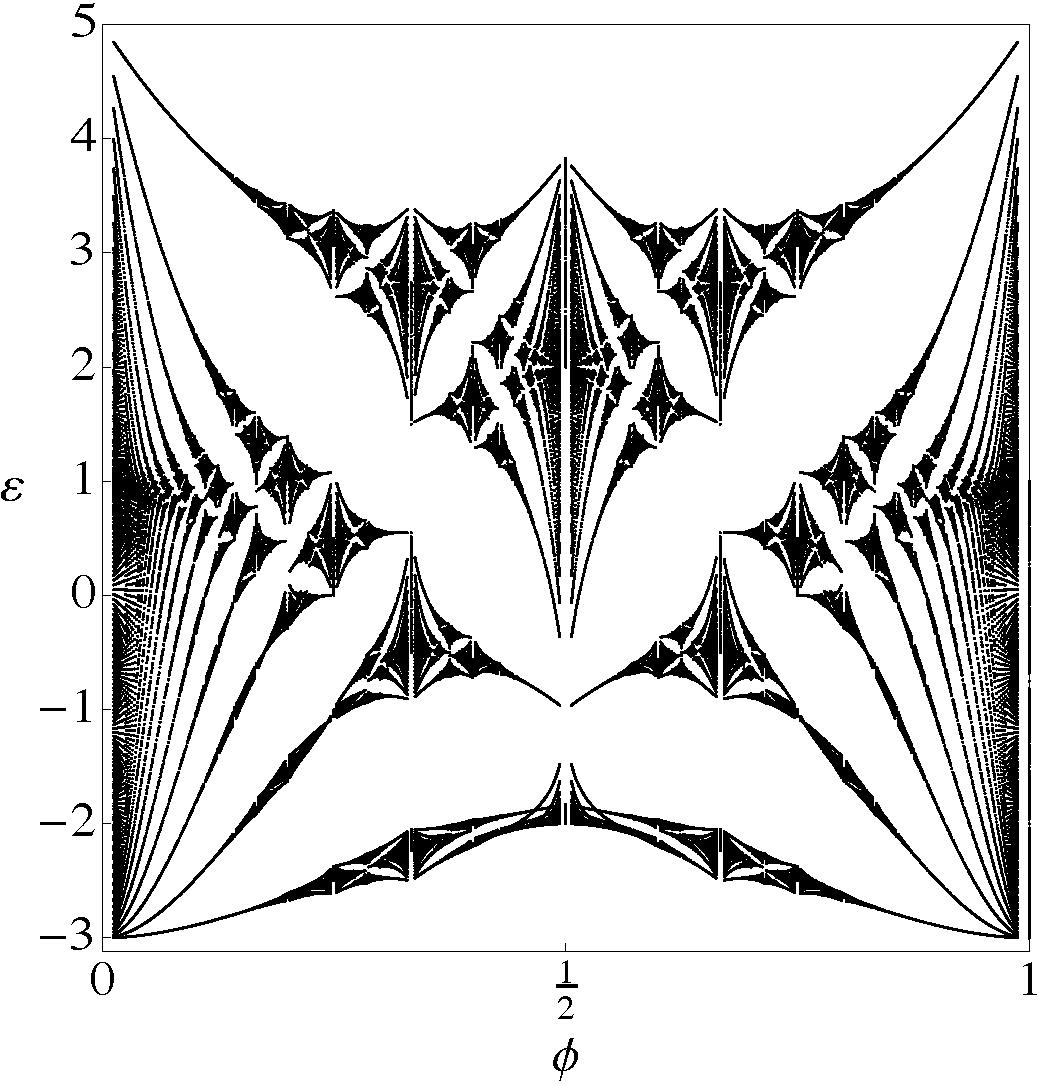
\includegraphics[width=1.45in]{/Users/dbauer/Physics/Manuscripts/quartic/quartic-butterfly-2.pdf}\label{fig:butterfly}}
% % \caption{Test}
% % \end{figure}


% \begin{figure}[bht]
% \centering
% \includegraphics[width=3.0in]{/Users/dbauer/Physics/Manuscripts/quartic/lattice-eval-2.pdf}
% \caption{\label{fig:ground-state} Energy in lowest quartic Hofstadter band at $\mathbf{k}=(0,0)$ for some rational values of flux per plaquette $\phi$. The red square shows the approximate lowest eigenvalue of the continuum Hamiltonian (\ref{eq:quartic-continuum-hamiltonian}).}
% \end{figure}

% As in the Hofstadter model, we can consider the small flux limit and find a corresponding continuum eigenvalue equation, approximating the finite difference
% \[
% \psi_{n+2} + \psi_{n-2} -4 \psi_{n+1} -4 \psi_{n-1} +6\psi_n \approx \frac{d^4\psi}{d x^4}.
% \]
% We then set the hopping strength so that $t_2 = -t_1/4$, and (\ref{eq-harper-2}) becomes
% \begin{align}
% &\frac{d^4\psi}{dx^4} - 8\cos(2 \pi \phi x) \psi(x)\nonumber \\*
%  + &2\cos\left[2\left(2 \pi \phi x\right)\right]\psi(x) = \left(4\frac{\varepsilon}{t_1}+6\right) \psi(x),
% \end{align}
% setting $k_y=0$ as discussed. Expanding the cosine term and defining $\omega \equiv 2\pi\phi/\phi_0$, $\tilde{\varepsilon} \equiv \varepsilon/t_1 + 3$, the eigenvalue equation becomes
% \[
% \frac{1}{4}\frac{d^4\psi}{dx^4} + \frac{1}{4}\omega^4 x^4 \psi(x) = \tilde{\varepsilon} \psi(x),
% \]
% the Schr{\"o}dinger equation for the stationary states of (\ref{eq:quartic-continuum-hamiltonian}) in the Landau gauge. We that note by introducing longer range hoppings of the same form (e.g., hopping three lattice spacings in the $x$ and $y$ directions), one can generate lattice models with continuum limit Hamiltonians $H \propto \bm{\pi}^{2n}$ for integral $n$. Additionally, choosing different hopping parameters in the $x$ and $y$ directions leads to anisotropic band mass.

% \section{Interactions and FQH states}
% To study the FQHE in this quartic model, we exactly diagonalize interactions projected to the lowest quartic Hofstadter band. We observed two different quantum Hall states, the $\nu = 1/2$ Laughlin state of bosons and the $\nu = 1/3$ Laughlin state of fermions. For each of these cases, we use $N_p = 8$ particles partially filling the lowest band on a lattice with periodic boundary conditions and topology of a torus. For the $\nu = 1/2$ case, we use a two-body repulsive delta function interaction, and place the particles on a lattice of $4 \times 4$ unit cells. We vary the flux per plaquette by increasing the size of each unit cell, using unit cells of dimension $m \times m$. For the $\nu = 1/3$ case, we use a lattice of $4 \times 6$ unit cells, with unit cell dimensions $3m \times 2m$.

% For each many-body ground state, we observe signatures of relevant FQH topological order in the energy and entanglement spectra, including a quasi-degenerate ground state with gapped excitations, $m$-fold degeneracy in the torus topology, and a gap in the particle entanglement spectrum. The many-body gap as a function of flux per plaquette is plotted in Figs. \ref{fig:boson-gap} and \ref{fig:fermion-gap} for bosons and fermions, respectively.

% We can also study the projection of interactions to the continuum bands directly by approximating these bands as mixtures of Landau levels. Starting from periodic Landau level states $\left|n, k\right>$ on a torus, we consider the single-particle states
% \begin{equation}
% \left|\psi,k\right> = c_0 \left|0, k\right> + c_4 \left|4, k\right>,
% \end{equation}
% where $c_0$, $c_4$ are the approximate overlaps defined in Sec. \ref{sec:intro-quartic}. We fill the orbitals with $N_p=8$ bosons at $\nu=1/2$ filling, and project a repulsive, two-body delta interaction. Diagonalizing this interaction yields a two-fold degenerate many-body ground state with gapped excitations. The many-body gap is displayed in Fig. \ref{fig:boson-gap} along with the gap of the corresponding lattice phase. The lattice gap does not converge to this approximate continuum value, which we attribute to our poor approximation of the single-particle ground state.

% %Many-body gaps as a function of flux per plaquette for Laughlin state of $N_{p}=8$ bosons at $\nu = 1/2$. (b). Laughlin state of $N_{p}=8$ fermions at $\nu = 1/3$. (c). Moore-Read state of $N_{p}=8$ bosons at $\nu = 1$.


% \begin{figure}[bht]
% \centering
% \includegraphics[width=2.9in]{/Users/dbauer/Physics/Manuscripts/quartic/fqh-gap-boson-2.pdf}
% \caption{\label{fig:boson-gap}Many-body gap as a function of flux per plaquette for Laughlin state of $N_{p}=8$ bosons at $\nu = 1/2$. The red square shows an approximate value for the many-body gap for bosons in the continuum ground state.}
% \end{figure}

% \begin{figure}[bht]
% \centering
% \includegraphics[width=2.9in]{/Users/dbauer/Physics/Manuscripts/quartic/fqh-gap-fermion.pdf}
% \caption{\label{fig:fermion-gap}Many-body gaps as a function of flux per plaquette for Laughlin state of $N_{p}=8$ fermions at $\nu = 1/3$.}
% \end{figure}


% % \subsection{Band geometry of the quartic Hofstadter model}
% As was done in \cite{Jackson:2015aa,Bauer:2016aa} for various lattice models, we can numerically study the geometry of the quartic Hofstadter model as a way to quantify deviations from lowest Landau level (LLL) behavior. The relationship between Chern band geometry and deviations from LLL physics was developed in \cite{Roy:2012vo} in terms of density operators projected to Chern bands. For $\phi=1/N$, the Chern number of each quartic Hofstadter band is 1. Deviations from the LLL can be measured by several band geometric quantities related to the Berry curvature and the Fubini-Study or quantum metric. In particular, inequalities relating the trace and determinant of the quantum metric to the Berry curvature are saturated in the LLL, and they are related to the closure of the algebra of projected density operators.

% In \cite{Bauer:2016aa}, the Brillouin zone average of the ``trace inequality'' $\left<T\right>$ was shown to be related to the stability, especially in bands in which Berry curvature and quantum metric fluctuations can be neglected. In the Hofstadter model, $\left<T\right>$ vanishes in the small flux limit corresponding to the saturation of the inequality in the lowest Landau level. By contrast, we observe numerically that $\left<T\right>$ remains finite for the small flux limit quartic Hofstadter model, as is the case in, for example, higher Landau levels. We also note that the many-body gap of the quartic Hofstadter model appears correlated with $\left<T\right>$, as seen in Figs. \ref{fig:tr-gap} although the functional dependence differs from that in the Hofstadter model.

% \begin{figure}[bht]
% \centering
% \includegraphics[width=2.9in]{/Users/dbauer/Physics/Manuscripts/quartic/gap-trace.png}
% \caption{\label{fig:tr-gap}[Placeholder]}
% \end{figure}

% \section{Discussion}
% In summary, we have exhibited a lattice model with a quartic Hamiltonian as its continuum limit, providing an example of continuum single-particle bands distinct from Landau levels that are capable of hosting the FQHE. 

% The question of whether a generic picture of the stability of FCIs exists remains open, and one ideally would like to develop some means to calculate properties of the many-body FQH state from single particle bands. An analog of the Girvin-MacDonald-Platzman calculation of the many-body gap extended to Chern bands would be a useful tool.

% Another interesting open question is what if any connection exists between the geometry of Chern bands and other geometric properties of QH states, for example the Hall viscosity.
% [...]

% \begin{acknowledgments}
% D.B. thanks R. Snively and F. Harper for helpful conversations, and T.S. Jackson for collaboration during this work and for contributing code used in this paper.
% \end{acknowledgments}

\bibliography{quartic-2}
% \bibliography{hofstadter-manual}

\end{document}


